\documentclass{TIJMUjiaoanSY}
\pagestyle{empty}


\begin{document}


%课程名称
\kecheng{系统生物学}
%实验名称
\shiyan{实验二\ 外显子组测序数据的处理}
%教师姓名
\jiaoshi{伊现富}
%职称
\zhicheng{讲师}
%教学日期(格式:XXXX年XX月XX日XX时-XX时)
\riqi{2016年10月20日13:30-16:30}
%授课对象(格式:XXX系XXXX年级XX班(硕/本/专科))
\duixiang{生物医学工程与技术学院2013级生信班(本)}
%实验人数
\renshu{28}
%实验类型
\leixing{验证型}
%实验分组
\fenzu{一人一机}
%学时数
\xueshi{3}
%教材版本
\jiaocai{系统生物学实验讲义(自编教材)}


%教案首页
\firstHeader
\maketitle
\thispagestyle{empty}

\mudi{
\begin{itemize}
  \item 掌握外显子组测序数据的分析流程。
  \item 熟悉BWA、SAMtools、SnpEff等工具的使用方法。
  \item 熟悉Galaxy的使用方法。
  \item 了解存储变异信息的VCF格式。
\end{itemize}
}

\fenpei{
\begin{itemize}
  \item (10')分析流程:回顾外显子组测序数据分析的基本流程。
  \item (10')常用工具:回顾总结外显子组测序数据分析中的常用工具。
  \item (10')VCF格式:回顾存储变异信息的VCF格式。
  \item (120')实验操作:从单端测序的外显子组测序数据中提取变异并进行注释。
\end{itemize}
}

\cailiao{
\begin{itemize}
  \item 实验材料:以FASTQ格式存储的单端外显子组测序数据。
  \item 主要仪器:联网的计算机。
  \item 分析工具:Galaxy,BWA,SAMtools,SnpEff。
\end{itemize}
}

\zhongdian{
\begin{itemize}
  \item 难点:VCF格式;解决策略:通过实例进行讲解。
  \item 重点:BWA、SAMtools和SnpEff的使用;解决策略:根据资料进行学习,通过练习熟练掌握。
\end{itemize}
}

\sikao{
\begin{itemize}
  \item 总结外显子组测序数据的分析流程。
  \item 列举外显子组测序数据分析中的常用工具。
  \item 解释存储变异信息的VCF格式。
\end{itemize}
}

\cankao{
\begin{itemize}
  \item BWA
  \item SAMtools
  \item SnpEff
  \item Galaxy
\end{itemize}
}

\firstTail


%教案续页
\newpage
\otherHeader

\noindent
\begin{enumerate}
  \item 分析流程(10分钟)
    \begin{figure}[ht]
      \centering
      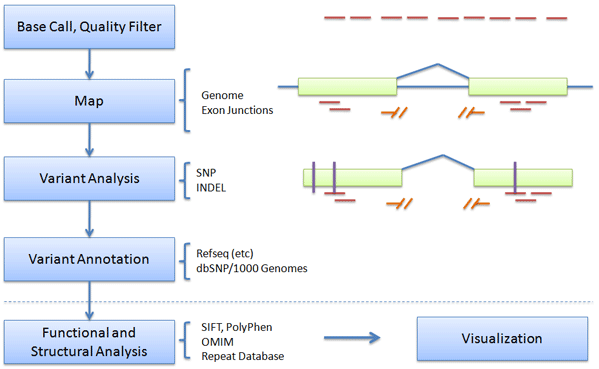
\includegraphics[width=0.9\textwidth]{c2.exome.bx.01.png}
    \end{figure}

  \item 常用工具(10分钟)
    \begin{itemize}
\parpic[fr]{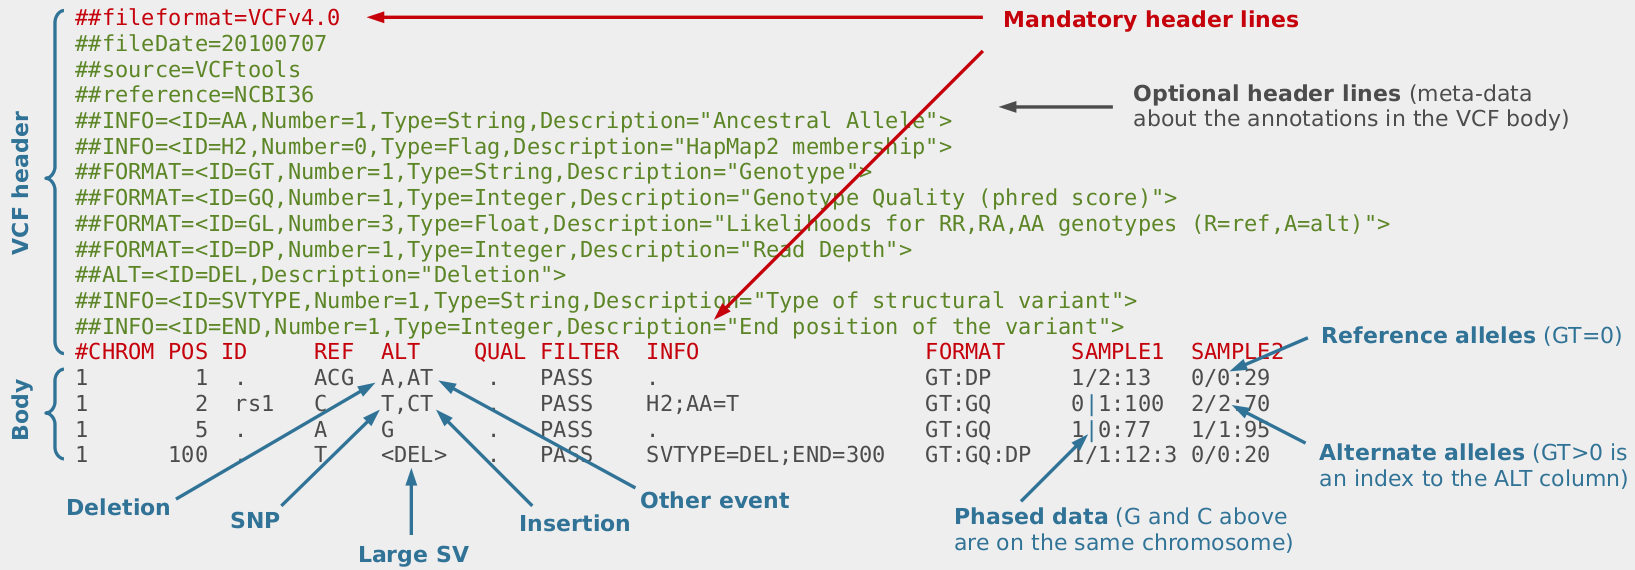
\includegraphics[width=11cm,height=6cm]{c2.format.vcf.05.png}}
      \item BWA: mapping reads against a reference genome
      \item Bowtie: an ultrafast, memory-efficient short read aligner
      \item SAMtools: interacting with high-throughput sequencing data
      \item VarScan: detect variants in NGS data
      \item SnpEff: genetic variant annotation and effect prediction toolbox
      \item ANNOVAR: functionally annotate genetic variants
    \end{itemize}

  \item VCF格式(10分钟)

  \item 实验操作(120分钟)
    \begin{enumerate}
      \item Upload data to Galaxy\textcolor{red}{(比较导入数据的不同方法;注意参数的设定)}
      \item Checking read quality with FastQC; Preprocessing\textcolor{red}{(参照实验一)}
      \item Map with BWA\textcolor{red}{(可以尝试一下其他类似工具)}
      \item Statistics with SAMtools\textcolor{red}{(可以尝试一下其他类似工具)}
      \item Call variants\textcolor{red}{(比较MPileup和Varscan的结果)}
      \item Annotate variants\textcolor{red}{(尝试不同的工具并比较结果)}
      \item Filter variants\textcolor{red}{(摸索阈值,尝试工具)}
    \end{enumerate}
\end{enumerate}


\otherTail


\end{document}

